%%%%%%%%%%%%%%%%%%%%%%%%%%%%%%%%%%%%%%%%%
% Beamer Presentation
% LaTeX Template
% Version 1.0 (10/11/12)
%
% This template has been downloaded from:
% http://www.LaTeXTemplates.com
%
% License:
% CC BY-NC-SA 3.0 (http://creativecommons.org/licenses/by-nc-sa/3.0/)
%
%%%%%%%%%%%%%%%%%%%%%%%%%%%%%%%%%%%%%%%%%

%----------------------------------------------------------------------------------------
%	PACKAGES AND THEMES
%----------------------------------------------------------------------------------------

\documentclass{beamer}

\mode<presentation> {

% The Beamer class comes with a number of default slide themes
% which change the colors and layouts of slides. Below this is a list
% of all the themes, uncomment each in turn to see what they look like.

%\usetheme{default}
%\usetheme{AnnArbor}
%\usetheme{Antibes}
%\usetheme{Bergen}
%\usetheme{Berkeley}
%\usetheme{Berlin}
%\usetheme{Boadilla}
%\usetheme{CambridgeUS}
%\usetheme{Copenhagen}
%\usetheme{Darmstadt}
%\usetheme{Dresden}
%\usetheme{Frankfurt}
%\usetheme{Goettingen}
%\usetheme{Hannover}
%\usetheme{Ilmenau}
%\usetheme{JuanLesPins}
%\usetheme{Luebeck}
\usetheme{Madrid}
%\usetheme{Malmoe}
%\usetheme{Marburg}
%\usetheme{Montpellier}
%\usetheme{PaloAlto}
%\usetheme{Pittsburgh}
%\usetheme{Rochester}
%\usetheme{Singapore}
%\usetheme{Szeged}
%\usetheme{Warsaw}

% As well as themes, the Beamer class has a number of color themes
% for any slide theme. Uncomment each of these in turn to see how it
% changes the colors of your current slide theme.

%\usecolortheme{albatross}
%\usecolortheme{beaver}
%\usecolortheme{beetle}
%\usecolortheme{crane}
%\usecolortheme{dolphin}
%\usecolortheme{dove}
%\usecolortheme{fly}
%\usecolortheme{lily}
%\usecolortheme{orchid}
%\usecolortheme{rose}
%\usecolortheme{seagull}
%\usecolortheme{seahorse}
%\usecolortheme{whale}
%\usecolortheme{wolverine}

%\setbeamertemplate{footline} % To remove the footer line in all slides uncomment this line
%\setbeamertemplate{footline}[page number] % To replace the footer line in all slides with a simple slide count uncomment this line

%\setbeamertemplate{navigation symbols}{} % To remove the navigation symbols from the bottom of all slides uncomment this line
}

\AtBeginSection[]{
  \begin{frame}
  \vfill
  \centering
  \begin{beamercolorbox}[sep=8pt,center,shadow=true,rounded=true]{title}
    \usebeamerfont{title}\insertsectionhead\par%
  \end{beamercolorbox}
  \vfill
  \end{frame}
}

\setbeamertemplate{headline}
{
  \leavevmode%
  \hbox{%
  \begin{beamercolorbox}[wd=.5\paperwidth,ht=2.25ex,dp=1ex,right]{section in head/foot}%
    \usebeamerfont{section in head/foot}\thesection\ \insertsectionhead\hspace*{2ex}
  \end{beamercolorbox}%
  \begin{beamercolorbox}[wd=.5\paperwidth,ht=2.25ex,dp=1ex,left]{subsection in head/foot}%
    \usebeamerfont{subsection in head/foot}\hspace*{2ex}\insertsubsectionhead
  \end{beamercolorbox}}%
  \vskip0pt%
}

\usepackage[brazilian]{babel}
\usepackage[utf8]{inputenc}
\usepackage{graphicx} % Allows including images
\usepackage{booktabs} % Allows the use of \toprule, \midrule and \bottomrule in tables
\usepackage[utf8]{inputenc}
\usepackage{xcolor}
\usepackage{tabularx}
\usepackage{amsmath}
\usepackage{pgfgantt}
\usepackage{hyperref}
\hypersetup{
	   colorlinks=true,    
       urlcolor=cyan,
}
\usepackage{tikz}
\usetikzlibrary{shapes,arrows}
\tikzstyle{decision} = [diamond, draw, fill=blue!20, 
    text width=4.5em, text badly centered, node distance=3cm, inner sep=0pt]
\tikzstyle{block} = [rectangle, draw, fill=blue!20, 
    text width=5em, text centered, rounded corners, minimum height=4em]
\tikzstyle{line} = [draw, -latex']
\tikzstyle{cloud} = [draw, ellipse,fill=red!20, node distance=3cm,
    minimum height=2em]

\newcommand{\norm}[1]{\left\lVert#1\right\rVert}
%----------------------------------------------------------------------------------------
%	TITLE PAGE
%----------------------------------------------------------------------------------------

\title[Trabalho de Graduação 1]{Compressão de Imagens com Perdas usando Redes Neurais} % The short title appears at the bottom of every slide, the full title is only on the title page

\author[Raphael Soares Ramos]{Raphael Soares Ramos} % Your name
\institute[UnB] % Your institution as it will appear on the bottom of every slide, may be shorthand to save space
{
Universidade de Brasília \\ % Your institution for the title page
\medskip
\textit{raphael.soares.1996@gmail.com} % Your email address
}
\date{\today} % Date, can be changed to a custom date

\begin{document}

\begin{frame}
\titlepage % Print the title page as the first slide
\end{frame}

\begin{frame}[allowframebreaks]
\frametitle{Overview} % Table of contents slide, comment this block out to remove it
\tableofcontents % Throughout your presentation, if you choose to use \section{} and \subsection{} commands, these will automatically be printed on this slide as an overview of your presentation
\end{frame}

%----------------------------------------------------------------------------------------
%	PRESENTATION SLIDES
%----------------------------------------------------------------------------------------

%------------------------------------------------
\section{Introdução}
%------------------------------------------------
\subsection{Definições}
%------------------------------------------------
\begin{frame}
\frametitle{Codificação de Dados}
\begin{itemize}
\item Transformação feita nos dados para atingir um certo objetivo.
\item Compressão (redução do comprimento) vs. Criptografia (proteger sigilo ou integridade do que os dados significam).
\end{itemize}
\end{frame}
%------------------------------------------------
\begin{frame}
\frametitle{Compressão de Dados}
\begin{itemize}
\item Processo de codificar uma determinada informação utilizando uma menor representação.
\item Arte ou ciência de representar informação de forma compacta~\cite{book_compression}.
\item Representações compactas são criadas identificando e usando estruturas existentes nos dados para que seja possível extrair redundâncias nos dados~\cite{book_compression}.
\end{itemize}
\end{frame}
%------------------------------------------------
\begin{frame}
\frametitle{Tipos de Compressão}
\begin{itemize}
\item Sem perdas (Lossless):
\begin{itemize}
\item $x = \hat{x}$
\end{itemize}
\item Com perdas (Lossy):
\begin{itemize}
\item $x \neq \hat{x}$
\end{itemize}
\end{itemize}
\begin{tikzpicture}[node distance = 2.5cm, auto]
    % Place nodes
    \node [block] (input) {Sinal de entrada x};
    \node [block, right of=input] (coder) {Codificador};
    \node [block, right of=coder] (code) {Sinal codificado};
    \node [block, right of=code] (decoder) {Decodifi-\\cador};
    \node [block, right of=decoder] (output) {Sinal decodificado $\hat{x}$};
    % Draw edges
    \path [line] (input) -- (coder);
    \path [line] (coder) -- (code);
   	\path [line] (code) -- (decoder);
    \path [line] (decoder) -- (output);
\end{tikzpicture}   
\end{frame}
%------------------------------------------------
\subsection{Motivação}
%------------------------------------------------
\begin{frame}
\frametitle{Porquê comprimir}
\begin{itemize}
    \item Geração e uso cada vez maior de dados digitais (muitos são redundantes e irrelevantes para determinadas aplicações).
    \item Representar digitalmente 1 segundo de vídeo sem compressão usando o formato CCIR 601 requer mais de 20 \textit{megabytes} de armazenamento ou 160 megabits para transmissão~\cite{book_compression}.
    \item Imagem Monocromática com resolução $512\times512$: $Taxa = \dfrac{512\cdot512\cdot8}{10^6} = 2.097 Mbits$.
    \item Aumentar capacidade de armazenamento e de transmissão de um sistema.
    \item Para serviços de streaming de mídia como Netflix, não usar compressão não é uma opção.
\end{itemize}
\end{frame}
%------------------------------------------------
\subsection{Compressão de Imagens}
%------------------------------------------------
\begin{frame}
\frametitle{Medidas de Desempenho em Compressão de Imagens}
\begin{itemize}
    \item Representar com o menor número possívels de bits, preservando a qualidade e a inteligibilidade necessárias à sua aplicação.
    \item Taxa vs. Distorção.
    \item \textit{Mean Squared Error} é uma medida de distorção.
    \begin{equation} MSE = \dfrac{1}{n}\sum_{n=1}^{N}{(x(n) - \hat{x}(n))}^2 \end{equation}
\end{itemize}
\end{frame}
%--------------------------------------------------
\begin{frame}
\frametitle{Algoritmos de Compressão de Imagens}
\begin{itemize}
    \item Exploram características imperfeitas da nossa percepção e propriedades estatísticas para fornecer resultados superiores quando comparados com métodos de compressão de dados genéricos.
    \item Examinada durante anos por pesquisadores e times como o \textit{Joint Pictures Experts Group}.
    \item Alguns métodos de compressão:
    \begin{enumerate}
    \item JPEG~\cite{jpeg}
    \item JPEG2000~\cite{jpeg2000}
    \item BPG~\cite{bpg}
    \item WebP~\cite{webp}
    \end{enumerate}
\end{itemize}
\end{frame}
%--------------------------------------------------
\begin{frame}
\frametitle{Elementos da Percepção Visual}
\begin{figure}
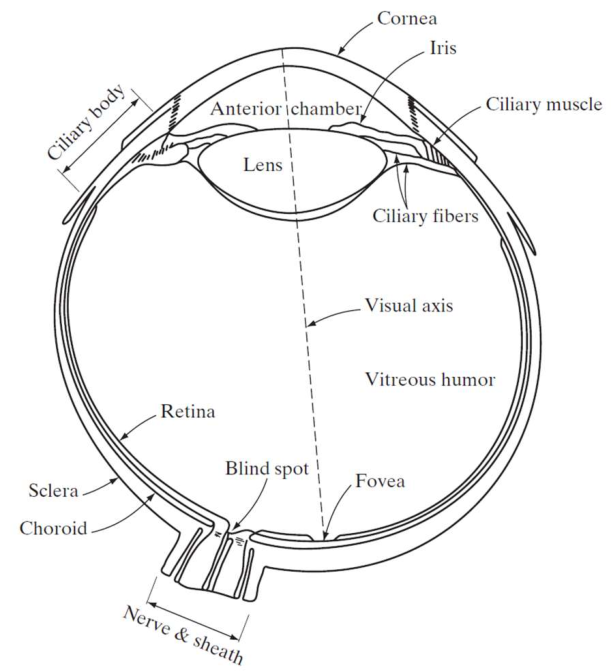
\includegraphics[width=0.4\textwidth]{figs/human_eye.pdf}
\caption{O olho humano é capaz de discriminar o brilho de uma imagem muito mais facilmente do que a sua informação de cor, pois existem cerca de 120 à 150 milhões de bastonetes distribuídos sobre a superfície da retina contra apenas 6 à 7 milhões de cones. Fonte:~\cite{ipi}}
\end{figure}
\end{frame}
%--------------------------------------------------
\begin{frame}
\frametitle{Elementos da Percepção Visual}
\begin{figure}
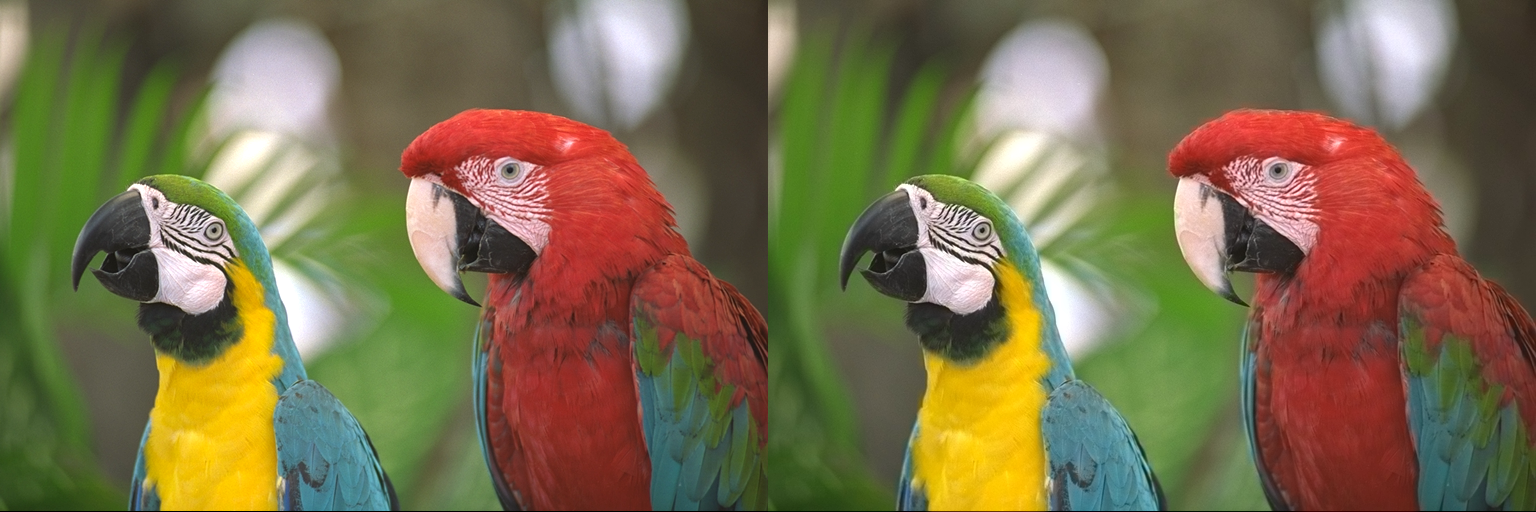
\includegraphics[width=\textwidth]{figs/image_comparison.png}
\caption{Imagem original 512x768 à esquerda (retirada de~\href{http://r0k.us/graphics/kodak/}{Kodak}) sem compressão e imagem (direita) gerada a partir da imagem original com dimensionalidade nos canais de crominância reduzida por um fator de 8 nas duas direções. Economia total de 2.1875 Kbytes para armazenamento!}
\label{fig:image_comp}
\end{figure}
\end{frame}
%--------------------------------------------------
\begin{frame}
\frametitle{Elementos da Percepção Visual}
\begin{figure}
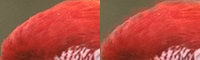
\includegraphics[width=\textwidth]{figs/zoom_image.png}
\caption{Versão com zoom da Figura~\ref{fig:image_comp}. Aqui é possível notar artefatos existentes devido à perda de informação.}
\end{figure}
\end{frame}
%------------------------------------------------
\subsection{Hipótese}
%------------------------------------------------
\begin{frame}
\frametitle{Hipótese}
\begin{itemize}
\item Nos últimos anos redes neurais profundas se tornaram a base dos resultados do estado da arte para diversas áreas
\item Deseja-se verificar se modelos baseados em \textit{autoencoders} convolucionais são competitivos com o clássico codec (codificador e decodificador) \textit{JPEG}.
\end{itemize}
\end{frame}
%--------------------------------------------------
\subsection{Objetivos}
%------------------------------------------------
\begin{frame}
\frametitle{Objetivos gerais e específicos}
\begin{itemize}
\item Foi proposto um \textit{autoencoder} convolucional que estenda a estrutura básica de um \textit{autoencoder}, gerando uma representação binária para a imagem.
\item Estudar propostas de compressão de imagens na literatura.
\item Avaliar o desempenho dos modelos propostos e do \textit{JPEG} em imagens de baixa resolução espacial.
\end{itemize} 
\end{frame}
%------------------------------------------------------
\section{Fundamentação Teórica}
%------------------------------------------------------
\subsection{JPEG}
%------------------------------------------------------
\begin{frame}
\frametitle{Formato de Arquivos}
\begin{itemize}
\item Arquivos comprimidos pelo método \textit{JPEG} são normalmente descritos no formato \textit{JPEG File Interchange Format (JFIF)}, que é uma limitação do padrão \textit{JPEG} completo (muitos espaços de cores e modos de operação).
\begin{enumerate}
\item Primeiro é feita conversão do espaço de cor para YCbCr.
\item É usado um fator para reduzir a quantidade de pixels nos componentes de crominância. Normalmente é usado um fator de 2 nas duas direções.
\end{enumerate}
\end{itemize} 
\end{frame}
%------------------------------------------------------
\begin{frame}
\frametitle{Funcionamento}
\begin{figure}
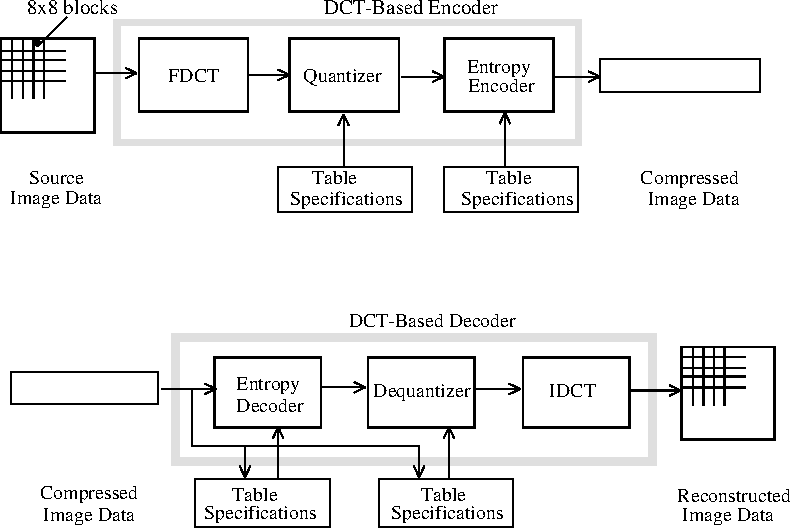
\includegraphics[width=0.75\textwidth]{figs/jpeg.pdf}
\caption{Diagrama geral que ilustra o funcionamento (codificação e decodificação) do método de compressão JPEG. Fonte:~\cite{jpeg}}
\end{figure} 
\end{frame}
%------------------------------------------------------
\begin{frame}
\frametitle{Transformada Discreta de Cosssenos (DCT)}
\begin{itemize}
\item Cada bloco 8x8 pode ser replicado por 64 (8x8) ondas de cossenos.
\item Analisa as frequências dos valores originais da imagem ao longo de cada linha e coluna usando um conjunto de ondas de cossenos oscilando em diferentes frequências e amplitudes. Cada bloco é representado usando estas ondas.
\end{itemize} 
\end{frame}
%------------------------------------------------------
\begin{frame}
\frametitle{Transformada Discreta de Cosssenos (DCT)}
\begin{figure}
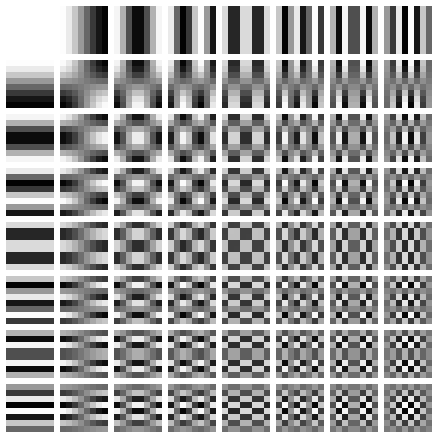
\includegraphics[width=0.48\textwidth]{figs/DCT-8x8.png}
\caption{64 ondas base de cossenos que produzem qualquer imagem 8x8. A DCT-II irá calcular os coeficientes - a contribuição de cada uma dessas ondas que somadas irão recriar a imagem perfeitamente. Fonte:~\cite{dct}}
\end{figure}
\end{frame}
%------------------------------------------------------
\newcommand\round[1]{\left[#1\right]}
\begin{frame}
\frametitle{Quantização}
\begin{itemize}
\item Para o \textit{encoder} será usada a seguinte equação:
\begin{equation}\round{F^Q(u,v) = \dfrac{F(u,v)}{Q(u,v)}}\end{equation}
\begin{enumerate}
\item Parte em que há maior perda de informação da imagem.
\item Cada um dos 64 coeficientes DCT $F(u,v)$ são uniformemente quantizados em conjunto com uma tabela de quantização de 64 elementos, que é definida pelo nível de qualidade escolhido para a aplicação.
\item Remove altas frequências definindo altos valores para $Q(u,v)$ (passo de quantização)
\end{enumerate}
\item No final, para cada bloco 8 por 8 da imagem original, existirá uma matriz quantizada.
\end{itemize}
\end{frame}
%------------------------------------------------------
\begin{frame}
\frametitle{Codificação}
\begin{figure}
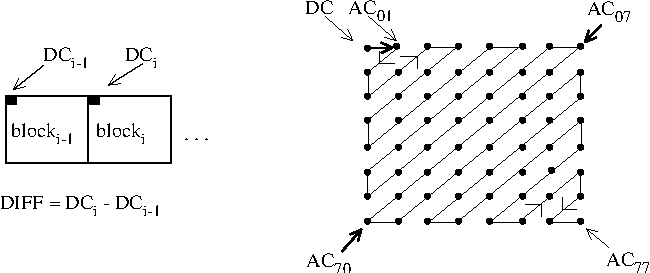
\includegraphics[width=\textwidth]{figs/coding_jpeg.pdf}
\caption{Codificação dos Direct Current (DC) coeficientes (esquerda) e sequência zig-zag usada para codificar todos os coeficientes (direita). Fonte:~\cite{jpeg}}
\end{figure}
\end{frame}
%------------------------------------------------------
\begin{frame}
\frametitle{O problema com o JPEG}
\begin{figure}

\includegraphics[width=\textwidth]{figs/text_jpeg.png}
\caption{Imagem de texto com e sem compressão. Fonte:~\cite{text_jpeg}}
\end{figure}
\end{frame}
%------------------------------------------------------
\subsection{Redes Neurais}
%------------------------------------------------------
\begin{frame}
\frametitle{Conceitos Básicos}
\begin{itemize}
\item Para muitas tarefas em inteligência artificial, é necessário extrair \textit{features} (características) dos dados.
\begin{enumerate}
\item As vezes é difícil saber quais \textit{features} devem ser extraídas.
\item Solução: aprender a representação dos dados (\textit{representation learning}).
\end{enumerate}
\item \textit{Deep learning} resolve o problema de \textit{representation learning} introduzindo representações que são expressadas em termos de outras representações mais simples.
\end{itemize} 
\end{frame}

%------------------------------------------------------
\begin{frame}
\frametitle{Conceitos Básicos}
\begin{itemize}
\item Redes neurais são algoritmos de \textit{deep learning} capazes de fazer predições aprendendo uma função que relaciona as características dos dados à respostas observadas/desejadas
\begin{enumerate}
\item Aproximadores universais de funções~\cite{nn_book}.
\item Funções de ativações permitem aprendizado de funções mais complexas. Mais comum é a \textit{ReLU}.
\begin{figure}
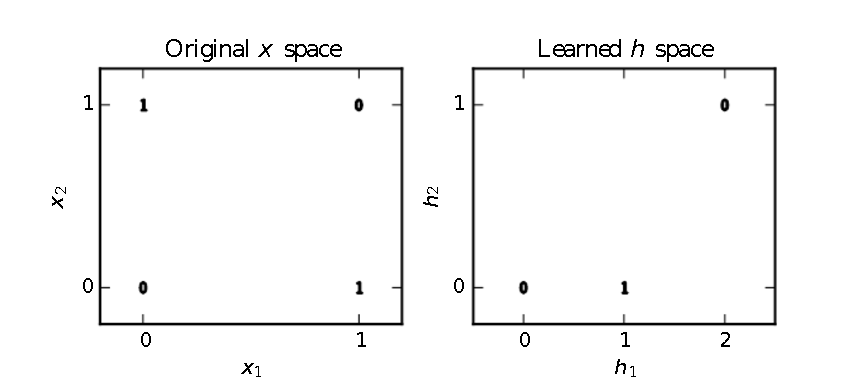
\includegraphics[width=0.7\textwidth]{figs/xor.pdf}
\caption{Um modelo linear aplicado diretamente à entrada original não pode implementar a função XOR. Fonte:~\cite{dl_book}}
\end{figure}
\end{enumerate}
\end{itemize}
\end{frame}
%------------------------------------------------------
\begin{frame}
\frametitle{Taxa de Aprendizagem}
\begin{equation} lr = baselr + (maxlr-baselr) max(0,\, 1-|itr/step - 2cycle + 1|) \gamma^{itr} \end{equation}
\begin{figure}
\includegraphics[width=\textwidth]{figs/exp.png}
\caption{Política exp\_range de \textit{learning rate} cíclica definida por~\cite{clr}. Fonte:~\cite{exp}}
\end{figure}
\end{frame}
%-----------------------------------------------------
\begin{frame}
\frametitle{Convoluções}
\begin{equation} g(x,\, y) \,=\, \sum_{s\, =\, -a}^{a}\, \sum_{t\, =\, -b}^{b}{w(s,t)f(x + s, y + t)} \end{equation}
\begin{figure}
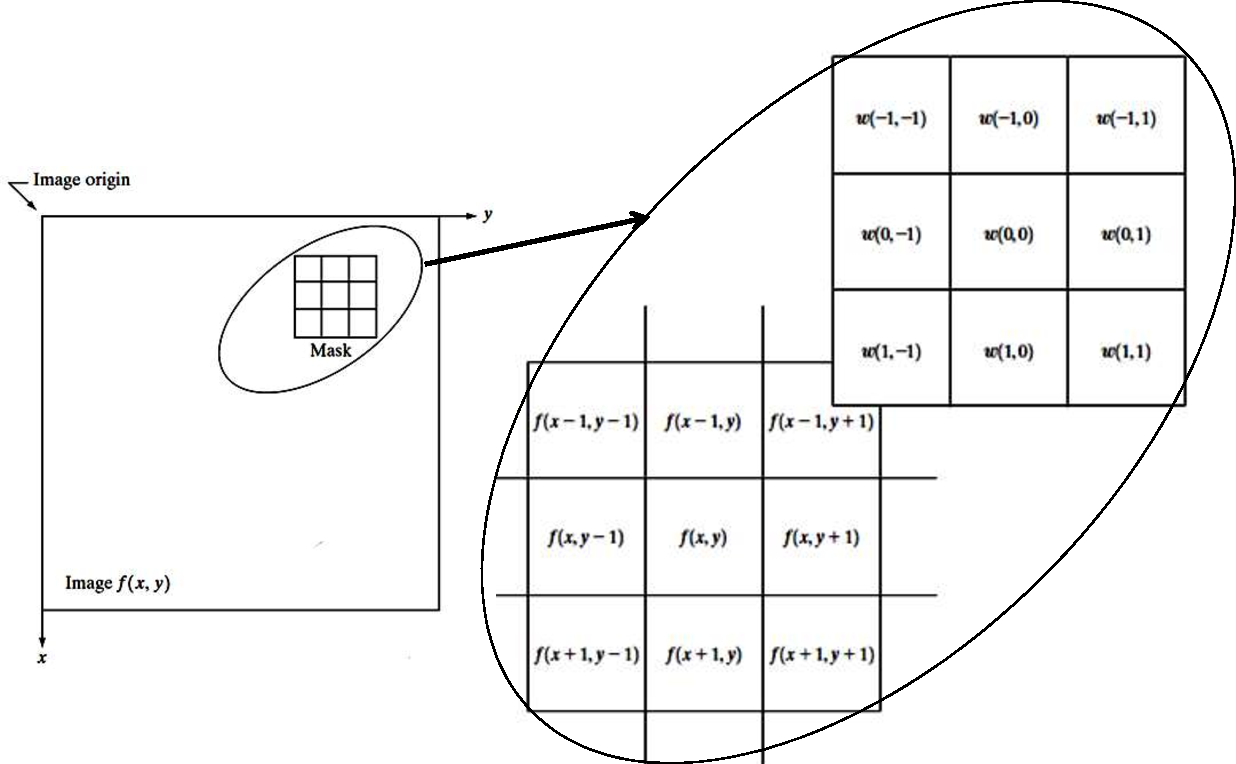
\includegraphics[width=0.62\textwidth]{figs/conv.pdf}
\caption{Operação de convolução. Fonte:~\cite{ipi}}
\end{figure}
\end{frame}
%------------------------------------------------------
\begin{frame}
\frametitle{Redes Neurais Convolucionais}
\begin{figure}
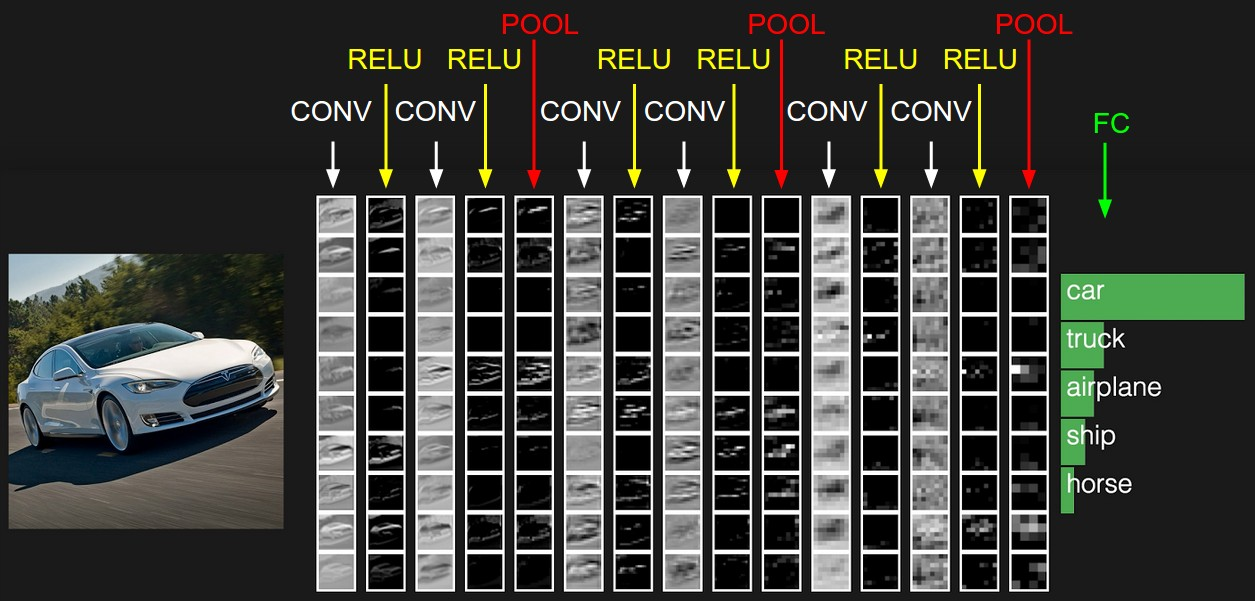
\includegraphics[width=\textwidth]{figs/convnet.jpeg}
\caption{Ilustração de uma rede neural convolucional. Fonte:~\cite{cnn}}
\end{figure}
\end{frame}
%------------------------------------------------------
\begin{frame}
\frametitle{Autoencoder}
\begin{figure}
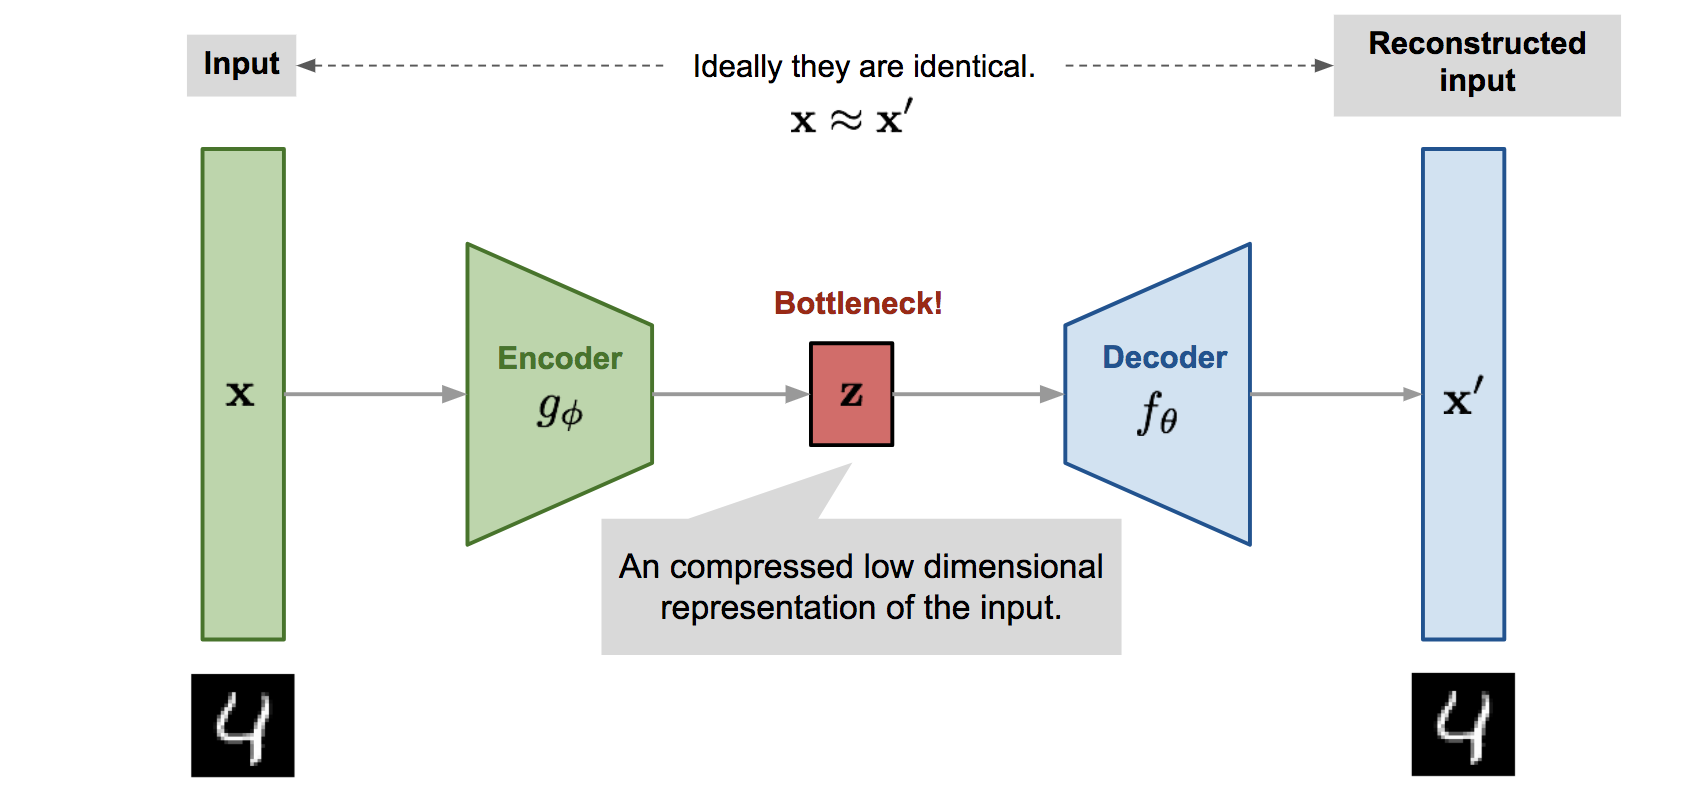
\includegraphics[width=\textwidth]{figs/ae-architecture.png}
\caption{Ilustração de um \textit{autoencoder}. Fonte:~\cite{ae}}
\end{figure}
\end{frame}
%------------------------------------------------------
\begin{frame}
\frametitle{Compressão de Imagens com Taxa Variável usando Redes Neurais Recorrentes~\cite{toderici}}
\begin{itemize}
\item Função de binarização $b(x)$:
\begin{equation} b(x) = x + \epsilon \,\in \{-1, 1\},\, \epsilon \sim \begin{cases} 
1 - x\, \text{ com probabilidade } \frac{1+x}{2},\\
-1 - x\, \text{ com probabilidade } \frac{1-x}{2},\\
\end{cases} \end{equation}
\item Binarizador: \begin{equation} B(x) = b(tanh(W^{bin}x + b^{bin})) \end{equation}
\item Em tempo de teste $b$ é substituída por:
\begin{equation}
b^{inf}(x) = \begin{cases}
-1,\, \text{ se } x < 0,\\
1,\, \text{ caso contrário. }\\
\end{cases}
\end{equation}
\item Autoencoder: $D(B(E(x)))$ 
\end{itemize}
\end{frame}
%------------------------------------------------------
\section{Metodologia}
%------------------------------------------------------
\subsection{Bases de Dados}
%------------------------------------------------------
\begin{frame}
\frametitle{Bases de Dados}
\begin{itemize}
\item Foram pegas imagens de \href{https://www.compression.cc/}{CLIC}, \href{https://data.vision.ee.ethz.ch/cvl/DIV2K/}{DIV2K} e \href{https://mmspg.epfl.ch/downloads/ultra-eye/}{EYE}.
\item Foram gerados 6,231,440 \textit{patches} com 32 pixels de largura e altura. Estes \textit{patches} foram divididos em 5 bases:
\begin{enumerate}
    \item \textbf{BD0}: formada por 1248978 de \textit{patches} que pertencem ao grupo dos 20\% com menor entropia;
    \item \textbf{BD1}: formada por 1251421 de \textit{patches} que pertencem ao grupo dos que estão na faixa 40\% à 60\% (porcentagem dada pelo \textit{patch} com maior entropia);
    \item \textbf{BD2}: formada por 1248725 de \textit{patches} que pertencem ao grupo dos 20\% com maior entropia;
    \item \textbf{BD3}: formada por 1247033 de \textit{patches} pegos de forma aleatória. Correspondem à 20\% do total.
    \item \textbf{BD4}: formada por 1246698 de \textit{patches}. 20\% do total retirados aleatoriamente dos 50\% de \textit{patches} com maior entropia.
\end{enumerate}
\end{itemize}
\end{frame}
%------------------------------------------------------
\begin{frame}
\frametitle{Bases de Dados}
\begin{figure}
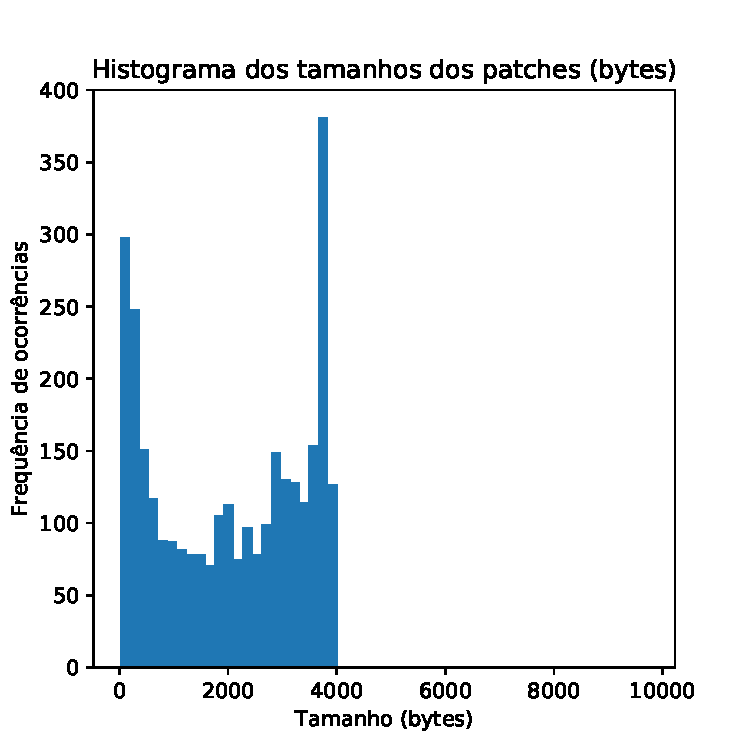
\includegraphics[width=0.5\textwidth]{figs/hist_all.pdf}
\caption{Histograma de todas as bases de dados.}
\end{figure}
\end{frame}
%------------------------------------------------------
\begin{frame}
\frametitle{Bases de Dados}
\begin{figure}
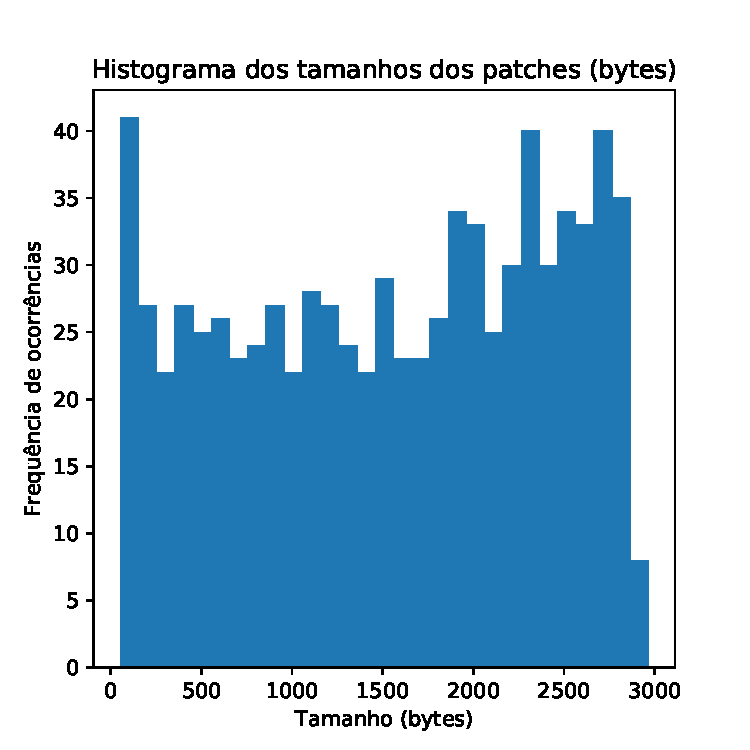
\includegraphics[width=0.5\textwidth]{figs/hist2.pdf}
\caption{Histograma da BD2.}
\end{figure}
\end{frame}
%------------------------------------------------------
\subsection{Modelos Desenvolvidos}
%------------------------------------------------------
\begin{frame}
\frametitle{Modelo 1}
\begin{figure}
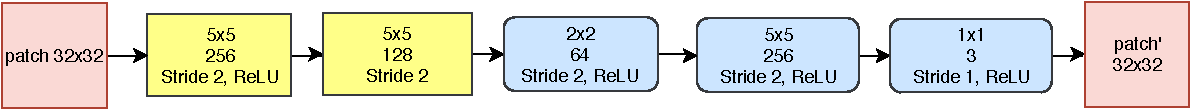
\includegraphics[width=\textwidth]{figs/conv_ae.pdf}
\caption{Ilustração do Modelo 1}
\end{figure}
\end{frame}

%------------------------------------------------------
\begin{frame}
\frametitle{Modelo 2}
\begin{figure}
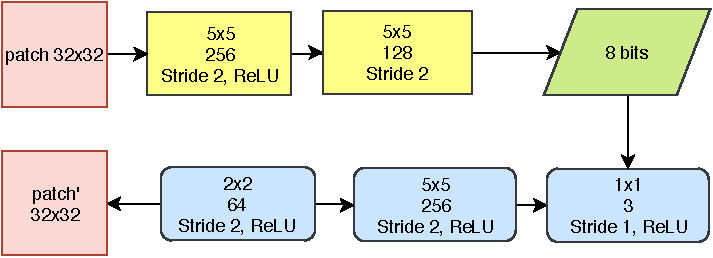
\includegraphics[width=\textwidth]{figs/conv_ae_bin.pdf}
\caption{Ilustração do Modelo 2.}
\end{figure}
\end{frame}

%------------------------------------------------------
\begin{frame}
\frametitle{Modelo 3}
\begin{figure}
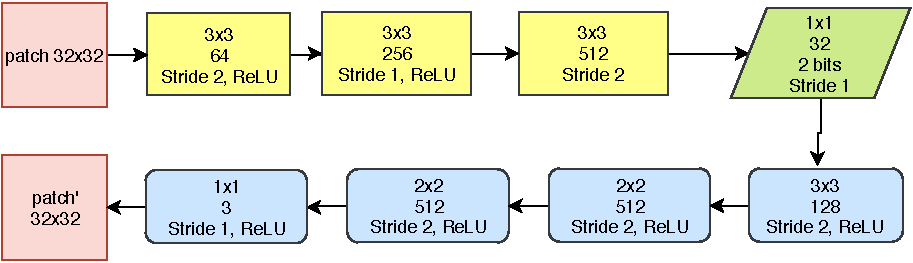
\includegraphics[width=\textwidth]{figs/toderici_model.pdf}
\caption{Ilustração do Modelo 3.}
\end{figure}
\end{frame}
%------------------------------------------------------
\section{Experimentos}
%------------------------------------------------------
\subsection{JPEG}
%------------------------------------------------------
\begin{frame}
\frametitle{Desempenho JPEG}
\begin{table}[]
\caption{Tabela contendo médias obtidas pelo \textbf{JPEG} em cada uma das bases de teste utilizadas}
\begin{tabular}{|l|l|l|l|l|l|}
\hline
\textbf{Bases}                                                                   & \textbf{BPP} & \textbf{PSNR} & \textbf{SSIM} & \textbf{MSSIM} & \textbf{Quality} \\ \hline
\textbf{\begin{tabular}[c]{@{}l@{}}CLIC Mobile test\\ (patches 32)\end{tabular}} & 8            & 44.23         & 0.98          & 0.99           & 94.06            \\ \hline
\textbf{CLIC Mobile test}                                                        & 2            & 39.58         & 0.96          & 0.99           & 88.69            \\ \hline
\textbf{Kodak}                                                                   & 2            & 36.77         & 0.95          & 0.99           & 85.91            \\ \hline
\textbf{BD0}                                                                     & 8            & 57.85         & 0.99          & 0.99           & 99.18            \\ \hline
\textbf{BD1}                                                                     & 8            & 42.94         & 0.97          & 0.99           & 95.94            \\ \hline
\textbf{BD2}                                                                     & 8            & 32.31         & 0.95          & 0.99           & 83.69            \\ \hline
\textbf{BD3}                                                                     & 8            & 43.84         & 0.96          & 0.99           & 93.94            \\ \hline
\textbf{BD4}                                                                     & 8            & 36.72         & 0.96          & 0.99           & 89.68            \\ \hline
\end{tabular}
\end{table}
\end{frame}
%------------------------------------------------------
\subsection{Modelo 1}
%------------------------------------------------------
\begin{frame}
\frametitle{Treino e Teste em todas as BDs}
\begin{table}[]
\caption{Tabela contendo o valor da \textit{PSNR}, em decíbeis, dos testes do \textbf{Modelo 1} com o uso do otimizador \textit{Adam} e \textit{learning rate} fixa. As linhas denotam a base de treino utilizada. As colunas denotam as bases de teste usadas para avaliação do modelo. O índice ``todas'' se refere ao uso de todas as imagens de todas as bases \textbf{BD} para treino}
\begin{tabular}{|l|l|l|l|l|l|}
\hline
\textbf{\begin{tabular}[c]{@{}l@{}}Treino (linhas) x \\Teste (colunas)\end{tabular}} & \textbf{BD0}   & \textbf{BD1}   & \textbf{BD2}   & \textbf{BD3}   & \textbf{BD4}   \\ \hline
\textbf{BD0}                                                                          & 49.66          & 38.07          & 26.34          & 38.05          & 31.13          \\ \hline
\textbf{BD1}                                                                          & 47.57          & 44.08          & 34.54          & 42.66          & 38.69          \\ \hline
\textbf{BD2}                                                                          & \textbf{53.69} & \textbf{51.16} & \textbf{44.07} & \textbf{50.06} & \textbf{47.14} \\ \hline
\textbf{BD3}                                                                          & 50.62          & 47.88          & 39.76          & 46.59          & 43.25          \\ \hline
\textbf{BD4}                                                                          & 47.30          & 46.98          & 41.10          & 45.63          & 43.75          \\ \hline
\textbf{Todas}                                                                        & 46.77          & 46.35          & 43.94          & 45.88          & 45.08          \\ \hline
\end{tabular}
\end{table}
\end{frame}
%------------------------------------------------------
\begin{frame}
\frametitle{Resultados}
\begin{table}[]
\caption{Tabela contendo o valor da \textit{PSNR}, em decíbeis, dos testes do Modelo 1 com o uso do otimizador \textit{Adam} e \textit{learning rate} fixa.}
\begin{tabular}{|l|l|}
\hline
\textbf{Treino (linhas) x Teste (coluna)}                                                              & \textbf{\textit{CLIC} Mobile test} \\ \hline
\textbf{BD0}                                                                                            & 34.77                    \\ \hline
\textbf{BD1}                                                                                            & 44.11                    \\ \hline
\textbf{BD2}                                                                                            & 48.97                   \\ \hline
\textbf{BD3}                                                                                            & 45.34                   \\ \hline
\textbf{BD4}                                                                                            & 42.42                    \\ \hline
\textbf{Todas}                                                                                          & 51.27                     \\ \hline
\textbf{Todas + CLIC Mobile train}                                                                      & \textbf{55.78}            \\ \hline
\textbf{\begin{tabular}[c]{@{}l@{}}Todas + Clic Mobile train + \\ Clic Professional train\end{tabular}} & 47.26                    \\ \hline
\textbf{CLIC Mobile Train}                                                                              & 46.63                   \\ \hline
\end{tabular}
\end{table}
\end{frame}
%------------------------------------------------------
\subsection{Modelo 2}
%------------------------------------------------------
\begin{frame}
\frametitle{Resultados}
\begin{table}[]
\caption{Tabela contendo os resultados do Modelo 2 para as métricas visuais \textit{PSNR}, \textit{SSIM} e \textit{MS-SSIM} a uma taxa nominal de 8 bits por pixel}
\begin{tabular}{|l|l|l|l|l|l|}
\hline
\textbf{\begin{tabular}[c]{@{}l@{}}Bases de Treino e\\ Teste\end{tabular}} & \textbf{BPP} & \textbf{PSNR} & \textbf{SSIM} & \textbf{MS-SSIM} & \textbf{Épocas} \\ \hline
\textbf{CLIC Mobile test}                                                       & 8            & 35.03         & 0.94          & 0.98           & 30              \\ \hline
\textbf{BD1}                                                               & 8            & 35.26         & 0.93          & 0.98           & 30              \\ \hline
\textbf{BD2}                                                               & 8            & 29.10         & 0.95          & 0.98           & 30              \\ \hline
\end{tabular}
\end{table}
\end{frame}
%------------------------------------------------------
\subsection{Modelo 3}
%------------------------------------------------------
\begin{frame}
\frametitle{Resultados}
\begin{table}[]
\caption{Tabela contendo os melhores resultados do Modelo 3}
\begin{tabular}{|l|l|l|l|l|}
\hline
\textbf{Bases}                                                                   & \textbf{BPP} & \textbf{PSNR} & \textbf{SSIM} & \textbf{MS-SSIM} \\ \hline
\textbf{\begin{tabular}[c]{@{}l@{}}CLIC Mobile test\\ (patches 32)\end{tabular}} & 2            & 33.75         & 0.92          & 0.97            \\ \hline
\textbf{\begin{tabular}[c]{@{}l@{}}Kodak\\ (patches 32)\end{tabular}}            & 2            & 31.46         & 0.88          & 0.96            \\ \hline
\textbf{BD0}                                                                     & 2            & 40.24         & 0.97          & 0.99            \\ \hline
\textbf{BD1}                                                                     & 2            & 35.00         & 0.91          & 0.98            \\ \hline
\textbf{BD2}                                                                     & 2            & 27.53         & 0.91          & 0.97            \\ \hline
\textbf{BD3}                                                                     & 2            & 33.27         & 0.91          & 0.97            \\ \hline
\textbf{BD4}                                                                     & 2            & 30.16         & 0.90          & 0.97            \\ \hline
\end{tabular}
\end{table}
\end{frame}
%------------------------------------------------------
\subsection{JPEG x Modelo 3}
%------------------------------------------------------
\begin{frame}
\frametitle{Curva Distorção vs. Taxa}
\begin{figure}
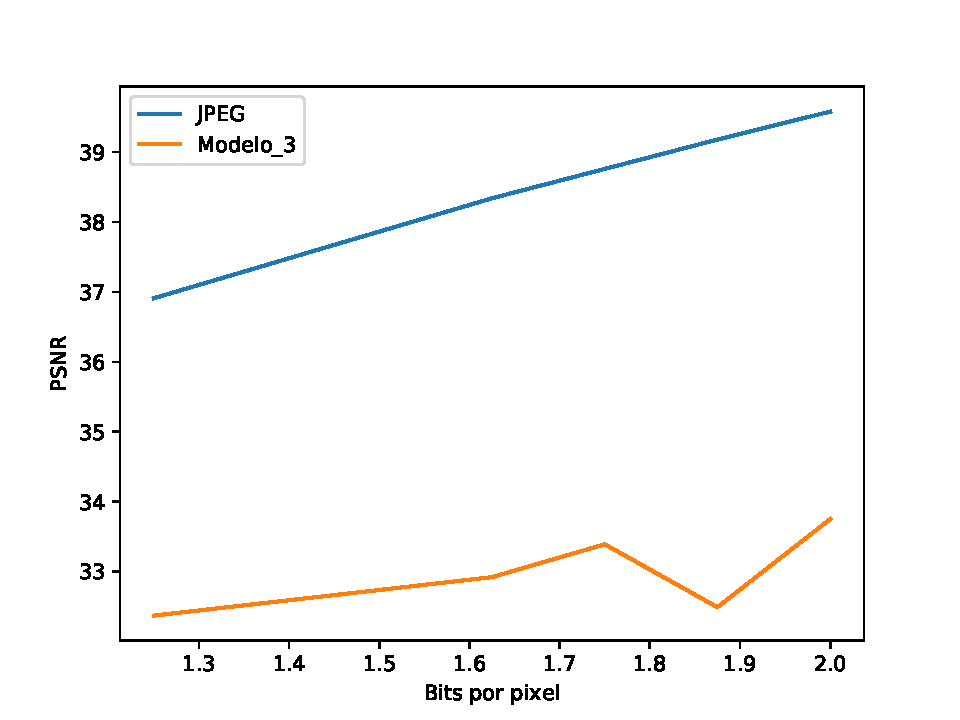
\includegraphics[width=0.7\textwidth]{figs/plots_psnr.pdf}
\caption{Comparação Modelo 3 e \textit{JPEG} na métrica PSNR.}
\end{figure}
\end{frame}
%------------------------------------------------------
\begin{frame}
\frametitle{Curva Distorção vs. Taxa}
\begin{figure}
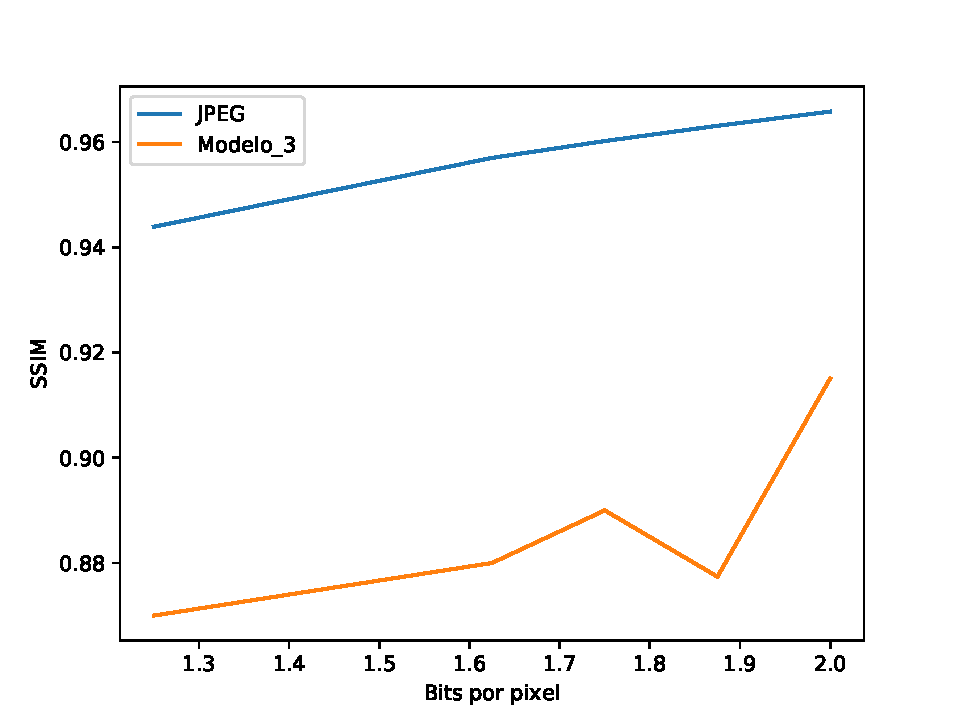
\includegraphics[width=0.7\textwidth]{figs/plots_ssim.pdf}
\caption{Comparação Modelo 3 e \textit{JPEG} na métrica SSIM.}
\end{figure}
\end{frame}
%------------------------------------------------------
\section{Conclusão}
%------------------------------------------------------
\begin{frame}
\frametitle{Limitações do Trabalho}
\begin{itemize}
\item Custo computacional superior aos codecs clássicos.
\item Algoritmos flexíveis, porém quantização é uma operação não diferenciável o que dificulta treinamento de redes neurais.
\end{itemize}
\end{frame}
%------------------------------------------------
\begin{frame}
\frametitle{Trabalho de Graduação 2}
\begin{figure}
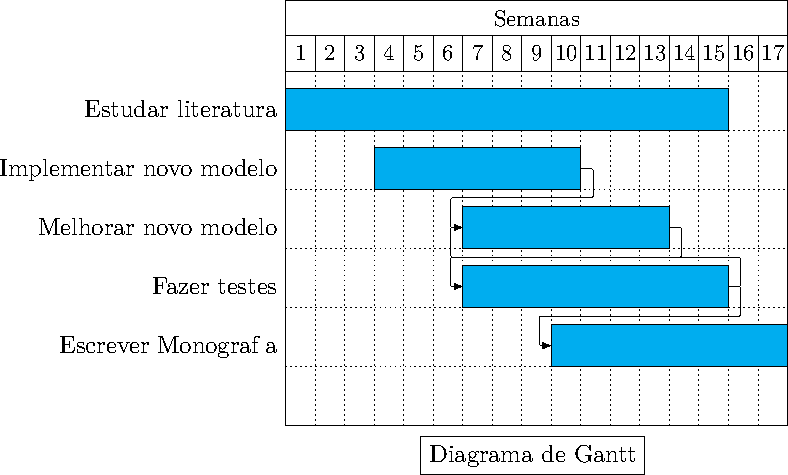
\includegraphics[width=\textwidth]{figs/diagram.pdf}
\caption{Atividades TG2.}
\end{figure}
\end{frame}
%------------------------------------------------

%----------------------------------------------------
%----------------------------------------------------
\begin{frame}[allowframebreaks]
\frametitle{References}
\footnotesize{
\begin{thebibliography}{99} % Beamer does not support BibTeX so references must be inserted manually as below
%----------------------------------------------------
\bibitem[Sayood et al. 2017]{book_compression} Khalid Sayood
\newblock Introduction to Data Compression
\newblock Morgan Kaufmann

\bibitem[G. K. Wallace et al. 1993]{jpeg} Gregory K. Wallace
\newblock The JPEG Still Picture Compression Stantard
\newblock In: IEEE Transactions on Consumer Electronics

\bibitem[C. {Christopoulos} et al. 2000]{jpeg2000} C. Christopoulos and A. Skodras and T. Ebrahimi
\newblock The JPEG2000 Still Image Coding System: An Overview
\newblock In: IEEE Transactions on Consumer Electronics

\bibitem[Bellard et al. 2019]{bpg} Fabrice Bellard
\newblock BPG image format
\newblock In: \href{https://bellard.org/bpg/}{BPG}

\bibitem[Google 2019]{webp} WebP
\newblock Compression Techniques 
\newblock In: \href{https://developers.google.com/speed/webp/docs/compression}{Compression}

\bibitem[Nielsen et. al 2015]{nn_book} Michael A. Nielsen
\newblock Neural Networks and Deep Learning
\newblock In: \href{http://neuralnetworksanddeeplearning.com/}{Determination Press}

\bibitem[Goodfellow et. al 2015]{dl_book} Ian Goodfellow and Yoshua Bengio and Aaron Courville
\newblock Deep Learning
\newblock In: \href{http://www.deeplearningbook.org}{MIT Press}

\bibitem[Zaghetto et. al 2018]{ipi} Alexandre Zaghetto
\newblock Introduction to Image Processing
\newblock In: \href{https://github.com/zaghetto/ImageProcessing}{GitHub Repository}

\bibitem[Wikimedia Commons 2015]{dct} Wikimedia Commons
\newblock Wikimedia Commons, The Free Media Repository
\newblock In: \href{https://commons.wikimedia.org/w/index.php?curid=10414002}{DCT Figure}

\bibitem[Mike Pound et. al 2015]{text_jpeg} Mike Pound - Computerphile
\newblock The Problem with JPEG - Computerphile
\newblock In: \href{https://youtu.be/yBX8GFqt6GA?t=48}{Computerphile Video}

\bibitem[Leslie et. al 2017]{clr} Leslie N. Smith
\newblock Cyclical Learning Rates for Training Neural Networks
\newblock In: Proceedings - IEEE Winter Conference on Applications of Computer Vision

\bibitem[Brad Kenstler et. al 2015]{exp} Brad Kenstler
\newblock Cyclical Learning Rate (CLR)
\newblock In: \href{https://github.com/bckenstler/CLR/}{GitHub Repository}

\bibitem[Lilain Weng et.al 2018]{ae} Lilian Weng
\newblock From Autoencoder to Beta-VAE
\newblock In: \href{https://lilianweng.github.io/lil-log/2018/08/12/from-autoencoder-to-beta-vae.html}{Blog}

\bibitem[CS231n Course Materials 2019]{cnn} CS231n
\newblock CS231n Convolutional Neural Networks for Visual Recognition
\newblock In: \href{http://cs231n.github.io/convolutional-networks}{CS231n}

\bibitem[Toderici et. al 2015]{toderici} Toderici, George and Vincent, Damien and Johnston, Nick and Jin Hwang, Sung and Minnen, David and Shor, Joel and Covell, Michele
\newblock Variable Rate Image Compression with Recurrent Neural Networks
\newblock In: ICLR 2016


\end{thebibliography}
}
\end{frame}



\end{document}